\begin{figure}
    \centering
    \small
    \hfill
    \begin{subfigure}{.5\linewidth}
        \centering
        \vspace{-0.5\baselineskip}
        \begin{tikzpicture}[hypergraph,xscale=.75,yscale=0.7,trim left=0cm,trim right=0cm]
            \node[vertex,label={west:$x_{\sf mid}$}] (mid) at (0, 0) {};
            \node[vertex,label={east:$x_{\sf kid}$}] (kid) at (-2.5, 0) {};
            \node[vertex,label={east:$x_{\sf k}$}] (k) at (-4, 0) {};

            \node[vertex,label={east:$x_{\sf pid}$}] (pid) at (0, -1.5) {};
            \node[vertex,label={east:$x_{\sf n}$}] (n) at (0, -2.5) {};
            
            \node[vertex,label={west:$x_{\sf cid}$}] (cid) at (2.5, 0) {};
            \node[vertex,label={west:$x_{\sf cc}$}] (cc) at (4, 0) {};
            
            \node[vertex,label={west:$x_{\sf t}$}] (t) at (0, 1) {};
        
            \begin{scope}[on background layer]
                    
                
                \newcommand*{\patht}{($(t) + (0,0.5)$)
        					to[out=180,in=180] ($(mid) + (0,-0.5)$)
        					to[out=0,in=0] ($(t) + (0,0.5)$)}

                \newcommand*{\pathmk}{	($(mid) + (0.25,0.25)$)
                    to[out=135,in=135] ($(kid) + (-0.25,-0.25)$)
                    to[out=-45,in=-45] ($(mid) + (0.25,0.25)$)}
                
                \newcommand*{\pathk}{($(kid) + (0.6,0)$)
        					to[out=90,in=90] ($(k) + (-0.5,0)$)
        					to[out=-90,in=-90] ($(kid) + (0.6,0)$)}

                \newcommand*{\pathci}{($(mid) + (0,0.5)$)
        					to[out=180,in=180] ($(pid) + (0,-0.5)$)
        					to[out=0,in=0] ($(mid) + (0,0.5)$)}

                \newcommand*{\pathn}{($(pid) + (0,0.5)$)
        					to[out=180,in=180] ($(n) + (0,-0.5)$)
        					to[out=0,in=0] ($(pid) + (0,0.5)$)}
                
                \newcommand*{\pathmc}{($(mid) + (-0.25,0.25)$)
                    to[out=45,in=45] ($(cid) + (0.25,-0.25)$)
                    to[out=-135,in=-135] ($(mid) + (-0.25,0.25)$)}
                
                \newcommand*{\pathcn}{($(cid) + (-0.5,0)$)
        					to[out=90,in=90] ($(cc) + (0.5,0)$)
        					to[out=-90,in=-90] ($(cid) + (-0.5,0)$)}
                
                \draw[hyperedge,looseness=1,draw=Red,fill=Red,fill opacity=.1] \patht;
                \draw[hyperedge,looseness=1,draw=Fuchsia,fill=Fuchsia,fill opacity=.1] \pathmk;
                \draw[hyperedge,looseness=1,draw=NavyBlue,fill=NavyBlue,fill opacity=.1] \pathk;
                \draw[hyperedge,looseness=1, draw=BurntOrange,fill=BurntOrange,fill opacity=.1] \pathmc;
                \draw[hyperedge,looseness=1, draw=TealBlue,fill=TealBlue,fill opacity=.1] \pathcn;
                \draw[hyperedge,looseness=1, draw=Gray,fill=Gray,fill opacity=.1] \pathci;
                \draw[hyperedge,looseness=1, draw=Thistle,fill=Thistle,fill opacity=.1] \pathn;
        
                \node[text=Red] at (0.75,1.25) {$R_{\sf t}$};
                \node[text=Fuchsia] at (-1.5,1) {$R_{\sf mk}$};
                \node[text=Cyan] at (-3.25,1) {$R_{\sf k}$};
                \node[text=BurntOrange] at (1.6,1) {$R_{\sf mc}$};
                \node[text=TealBlue] at (3.25,1) {$R_{\sf cn}$};
                \node[text=Gray] at (-1,-1) {$R_{\sf ci}$};
                \node[text=Thistle] at (-1,-2.25) {$R_{\sf n}$};
                
            \end{scope}
        \end{tikzpicture}
        \caption{Hypergraph}
        \label{fig:rel-dom-hg}
    \end{subfigure}
    \hfill
    \begin{subfigure}{.33\linewidth}
        \centering
        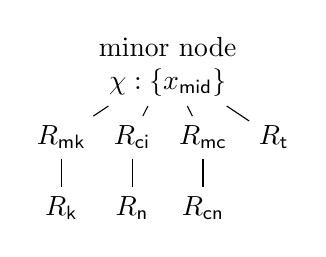
\begin{tikzpicture}[
			level distance=0.9cm,
			level 1/.style={sibling distance=0.9cm}
        ]
			\node[align=center] { minor node \\ $\chi: \{ x_{\sf mid} \}$ }
				child { node {$R_{\sf mk}$} edge from parent[-]
                    child { node {$R_{\sf k}$} edge from parent[-] }
                }
                child { node {$R_{\sf ci}$} edge from parent[-]
                    child { node {$R_{\sf n}$} edge from parent[-] }
                }
                child { node {$R_{\sf mc}$} edge from parent[-]
                    child { node {$R_{\sf cn}$} edge from parent[-] }
                }
                child { node {$R_{\sf t}$} edge from parent[-] };
                
		\end{tikzpicture}
        \caption{Meta-decomposition (simplified)}
        \label{fig:rel-dom-meta}
    \end{subfigure}
    \hfill \ 

    \begin{subfigure}{.3\linewidth}
        \centering
        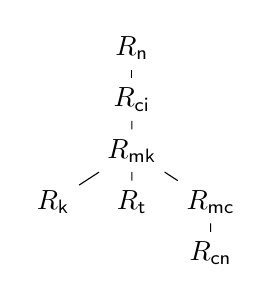
\begin{tikzpicture}[
			level distance=0.65cm,
			level 1/.style={sibling distance=1cm}
        ]
			\node { $R_{\sf n}$ }
				child { node {$R_{\sf ci}$} edge from parent[-]
                    child { node {$R_{\sf mk}$} edge from parent[-]
                        child { node {$R_{\sf k}$} edge from parent[-] }
                        child { node {$R_{\sf t}$} edge from parent[-] }
                        child { node {$R_{\sf mc}$} edge from parent[-]
                            child { node {$R_{\sf cn}$} edge from parent[-] }
                        }
                    }
                };
                
		\end{tikzpicture}
        \caption{Join tree inducing the width-1 plan in \cref{fig:rel-dom-w1}}
        \label{fig:rel-dom-jt}
    \end{subfigure}
    \hfill
    \begin{subfigure}{.33\linewidth}
        \centering
        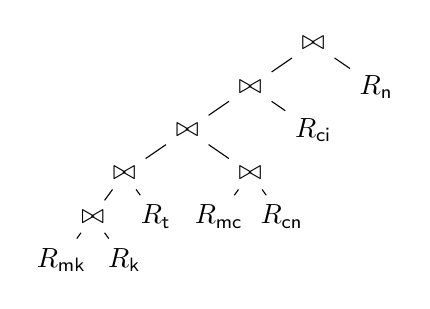
\begin{tikzpicture}[
			level distance=0.55cm,
            level 1/.style={sibling distance=1.6cm},
			level 2/.style={sibling distance=1.6cm},
            level 3/.style={sibling distance=1.6cm},
            level 4/.style={sibling distance=0.8cm}
        ]
			\node { $\bowtie$ }
                child { node {$\bowtie$} edge from parent[-]
                    child { node {$\bowtie$} edge from parent[-]
                        child { node {$\bowtie$} edge from parent[-]
            				child { node {$\bowtie$} edge from parent[-]
                                child { node {$R_{\sf mk}$} edge from parent[-] }
                                child { node {$R_{\sf k}$} edge from parent[-] }
                            }
                            child { node {$R_{\sf t}$} edge from parent[-] }
                        }
                        child { node {$\bowtie$} edge from parent[-]
                            child { node {$R_{\sf mc}$} edge from parent[-] }
                            child { node {$R_{\sf cn}$} edge from parent[-] }
                        }
                    }
                    child { node {$R_{\sf ci}$} edge from parent[-] } 
                }
                child { node {$R_{\sf n}$} edge from parent[-] };
		\end{tikzpicture}
        \caption{Optimal width-1 query plan, induced by the join tree in \cref{fig:rel-dom-jt}}
        \label{fig:rel-dom-w1}
    \end{subfigure}
    \hfill
    \begin{subfigure}{.3\linewidth}
        \centering
        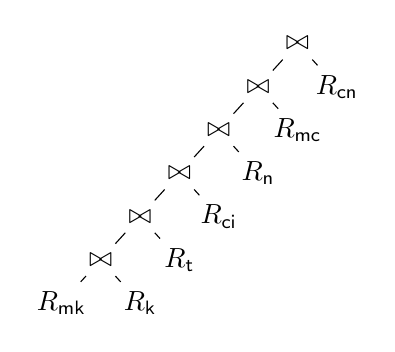
\begin{tikzpicture}[
			level distance=0.55cm,
			level 1/.style={sibling distance=1cm}
        ]
			\node { $\bowtie$ }
                child { node {$\bowtie$} edge from parent[-]
                    child { node {$\bowtie$} edge from parent[-]
                        child { node {$\bowtie$} edge from parent[-]
            				child { node {$\bowtie$} edge from parent[-]
                				child { node {$\bowtie$} edge from parent[-]
                                    child { node {$R_{\sf mk}$} edge from parent[-] }
                                    child { node {$R_{\sf k}$} edge from parent[-] }
                                }
                                child { node {$R_{\sf t}$} edge from parent[-] }
                            }
                            child { node {$R_{\sf ci}$} edge from parent[-] }
                        }
                        child { node {$R_{\sf n}$} edge from parent[-] }
                    }
                    child { node {$R_{\sf mc}$} edge from parent[-] }
                }
                child { node {$R_{\sf cn}$} edge from parent[-] };
		\end{tikzpicture}
        \caption{Optimal plan by dynamic programming, of width 2}
        \label{fig:rel-dom-duckdb}
    \end{subfigure}
    % \vspace{-0.75\baselineskip}
    \caption{The hypergraph, the meta-decomposition, the optimal width-1 query plan with the inducing join tree, and the optimal query plan (of width 2) found by dynamic programming, of the query JOB 17f in \cref{ex:rel-dom}}
    \label{fig:rel-dom}
\end{figure}
